\documentclass[11pt]{article}
\usepackage[margin=1in]{geometry}
\usepackage{amsmath, amsfonts, amssymb}
\usepackage{graphicx}
\usepackage{subcaption}
\usepackage{booktabs}
\usepackage{hyperref}

\title{\textbf{Supplementary Material: Ablation Studies for Second-Order PDE-Inspired Image Denoising}}

\author{
    \textbf{C V Rishi} \\ \small se23ucse044@mahindrauniversity.edu.in \and
    \textbf{G Rithvik} \\ \small se23ucse199@mahindrauniversity.edu.in \and
    \textbf{V Vivardhan} \\ \small se23ucse006@mahindrauniversity.edu.in \and
    \textbf{P Sai Sastha} \\ \small se23ucse141@mahindrauniversity.edu.in
}
\date{}

\begin{document}

\maketitle

\section{Introduction}

This supplementary document provides extended experimental results, ablation studies, and training logs for the second-order PDE-inspired unrolled network proposed in the main paper. We examine the sensitivity of the model to structural hyperparameters, including parameter learning, influence functions, and filter capacity.

\section{Architectural Ablations}

\subsection{Importance of Scalar Learning (Fixed Physics vs. Learned)}

Our model uses learnable scalars $(\alpha, \beta, \lambda)$ derived from the physical constants $\gamma$ and $\tau$. In the "Fixed Physics" experiment, we disable the optimizer for these scalars, forcing the network to adhere strictly to the theoretical discretization.

As shown in Table~\ref{tab:physics_ablation}, fixing the coefficients results in a massive performance drop ($-5.82$ dB). This confirms that while the hyperbolic PDE provides a strong architectural prior, the network must adapt its momentum and damping coefficients to compensate for the discrete nature of the unrolled stages and the learned filter-bank approximations.

\begin{table}[h]
	\centering
	\caption{Impact of Scalar Parameter Learning ($\sigma=25$)}
	\label{tab:physics_ablation}
	\begin{tabular}{l c c}
		\toprule
		Configuration      & Scalar Learning & PSNR (dB)      \\
		\midrule
		Fixed Physics      & No              & 20.48          \\
		Proposed (Greedy)  & \textbf{Yes}    & \textbf{26.30} \\
		\bottomrule
	\end{tabular}
\end{table}

\subsection{Influence Function Battle}

We compared the default Lorentzian influence function against Soft-Thresholding and Gaussian Derivatives. As summarized in Table~\ref{tab:phi_ablation}, Soft-Thresholding achieves the best stability and final PSNR. The Gaussian Derivative shows high performance in the first stage but exhibits slightly lower convergence in a greedy training setup.

\begin{table}[h]
	\centering
	\caption{Influence Function Comparison ($\sigma=25$)}
	\label{tab:phi_ablation}
	\begin{tabular}{l c}
		\toprule
		Influence Function $\phi(\cdot)$ & PSNR (dB)      \\
		\midrule
		Lorentzian                      & 26.29          \\
		Soft-Thresholding               & \textbf{26.30} \\
		Gaussian Derivative             & 25.96          \\
		\bottomrule
	\end{tabular}
\end{table}

\section{Model Capacity and Complexity}

\subsection{Filter Bank Width ($K$)}

We investigated the impact of the number of convolutional filters $K$ per stage. As shown in Table~\ref{tab:capacity_ablation}, increasing the capacity from $K=8$ to $K=48$ significantly improves the denoising quality. The model with $K=48$ achieves 26.39 dB, confirming that a wider filter bank is better at capturing the complex spatial statistics required for the learned diffusion operator.

\begin{table}[h]
	\centering
	\caption{Impact of Filter Bank Capacity ($K$) at Stage 5}
	\label{tab:capacity_ablation}
	\begin{tabular}{l c}
		\toprule
		Filters ($K$) & PSNR (dB)      \\
		\midrule
		8             & 25.94          \\
		24 (Base)     & 26.26          \\
		48            & \textbf{26.39} \\
		\bottomrule
	\end{tabular}
\end{table}

\subsection{Receptive Field (Filter Size)}

The spatial support of the learned filters determines the receptive field of each stage. We compared the baseline $7 \times 7$ filters with $3 \times 3$ and $9 \times 9$ variants. As seen in Table~\ref{tab:filter_ablation}, smaller filters result in a significant performance drop, whereas $9 \times 9$ filters provide a slight gain over the baseline. This suggests that the diffusion process requires a sufficiently large spatial context to effectively distinguish structural features from noise.

\begin{table}[h]
	\centering
	\caption{Impact of Filter Size at Stage 5}
	\label{tab:filter_ablation}
	\begin{tabular}{l c}
		\toprule
		Filter Size & PSNR (dB)      \\
		\midrule
		$3 \times 3$ & 25.94          \\
		$7 \times 7$ (Base) & 26.26 \\
		$9 \times 9$ & \textbf{26.31} \\
		\bottomrule
	\end{tabular}
\end{table}

\section{Damping Sensitivity and Stability}

The damping coefficient $\gamma$ controls the inertial behavior of the hyperbolic PDE. We tested $\gamma \in \{0.1, 0.5, 0.9\}$. As shown in Table~\ref{tab:gamma_ablation}, the model is relatively robust to the choice of $\gamma$ when scalars are learnable, as the network can adapt the momentum terms $(\alpha, \beta)$ to maintain stability and restoration quality.

\begin{table}[h]
	\centering
	\caption{Damping Coefficient Sensitivity ($\sigma=25$)}
	\label{tab:gamma_ablation}
	\begin{tabular}{l c}
		\toprule
		Damping $\gamma$ & PSNR (dB)      \\
		\midrule
		0.1             & \textbf{26.31} \\
		0.5 (Base)      & 26.26          \\
		0.9             & 26.27          \\
		\bottomrule
	\end{tabular}
\end{table}

\section{Training and Depth Analysis}

\subsection{Stage Saturation (Depth)}

We unrolled the PDE for $T \in \{3, 5, 15\}$ stages to find the saturation point. Table~\ref{tab:depth_ablation} shows that while performance increases with depth, the marginal gains diminish significantly after 10 stages. Stage 15 achieved 26.37 dB, only a 0.11 dB improvement over Stage 5, justifying our choice of $T=10$ for the main paper.

\begin{table}[h]
	\centering
	\caption{Impact of Depth (Number of Stages $T$)}
	\label{tab:depth_ablation}
	\begin{tabular}{l c}
		\toprule
		Stages ($T$) & PSNR (dB)      \\
		\midrule
		3            & 26.10          \\
		5 (Base)     & 26.26          \\
		15           & \textbf{26.37} \\
		\bottomrule
	\end{tabular}
\end{table}

\subsection{Loss Function Comparison (MSE vs. L1)}

Finally, we evaluated the impact of the loss function. While MSE is standard for maximizing PSNR, L1 loss is often preferred for edge preservation. Interestingly, in our unrolled hyperbolic framework, L1 loss led to a significantly higher PSNR of 27.47 dB. This suggests that the sparsity-promoting nature of L1 loss aligns well with the edge-preserving diffusion operator modeled by the PDE.

\begin{table}[h]
	\centering
	\caption{Loss Function Comparison at Stage 5}
	\label{tab:loss_ablation}
	\begin{tabular}{l c}
		\toprule
		Loss Function & PSNR (dB)      \\
		\midrule
		MSE (Base)    & 26.26          \\
		L1            & \textbf{27.47} \\
		\bottomrule
	\end{tabular}
\end{table}

\section{Dataset Generalization}

We observed that the model generalizes well across training sets. While initial runs on BSD400 yielded lower results, refined training demonstrates that BSD400 slightly outperforms FOE400 (Table~\ref{tab:dataset_ablation}).

\begin{table}[h]
	\centering
	\caption{Training Dataset Impact on CBSD68 Test Set}
	\label{tab:dataset_ablation}
	\begin{tabular}{l c c}
		\toprule
		Dataset & Stages & PSNR (dB)      \\
		\midrule
		BSD400  & 10     & \textbf{26.48} \\
		FOE400  & 7      & 26.30          \\
		\bottomrule
	\end{tabular}
\end{table}

\section{Training Duration and Overfitting}

We observed a non-intuitive relationship between the number of training epochs per stage and the final test PSNR. As shown in Table~\ref{tab:epoch_ablation}, increasing the training duration from 5 epochs to 10 epochs per stage actually led to a slight decrease in PSNR (26.48 dB to 26.35 dB).

\begin{table}[h]
	\centering
	\caption{Impact of Training Epochs per Stage on CBSD68 ($\sigma=25, T=10$)}
	\label{tab:epoch_ablation}
	\begin{tabular}{l c}
		\toprule
		Epochs per Stage & PSNR (dB)      \\
		\midrule
		5               & \textbf{26.48} \\
		10              & 26.35          \\
		\bottomrule
	\end{tabular}
\end{table}

This behavior suggests two potential phenomena:
\begin{enumerate}
    \item \textbf{Noise Overfitting}: In image denoising, the model may begin to learn the specific noise realizations present in the training patches rather than the underlying image manifold. Since we use a finite set of patches, excessive training allows the convolutional filters to "memorize" high-frequency noise patterns as if they were structural details.
    \item \textbf{Greedy Optimization Artifacts}: Because each stage is trained independently and frozen, over-optimizing an early stage might result in a denoised output that is "too clean" but mathematically ill-suited for further refinement by subsequent stages. A form of early stopping at each stage seems to provide a better initialization for the next step in the unrolled PDE.
\end{enumerate}

\section{Training Dynamics}

\begin{figure}[h]
    \centering
    \begin{subfigure}{0.48\linewidth}
        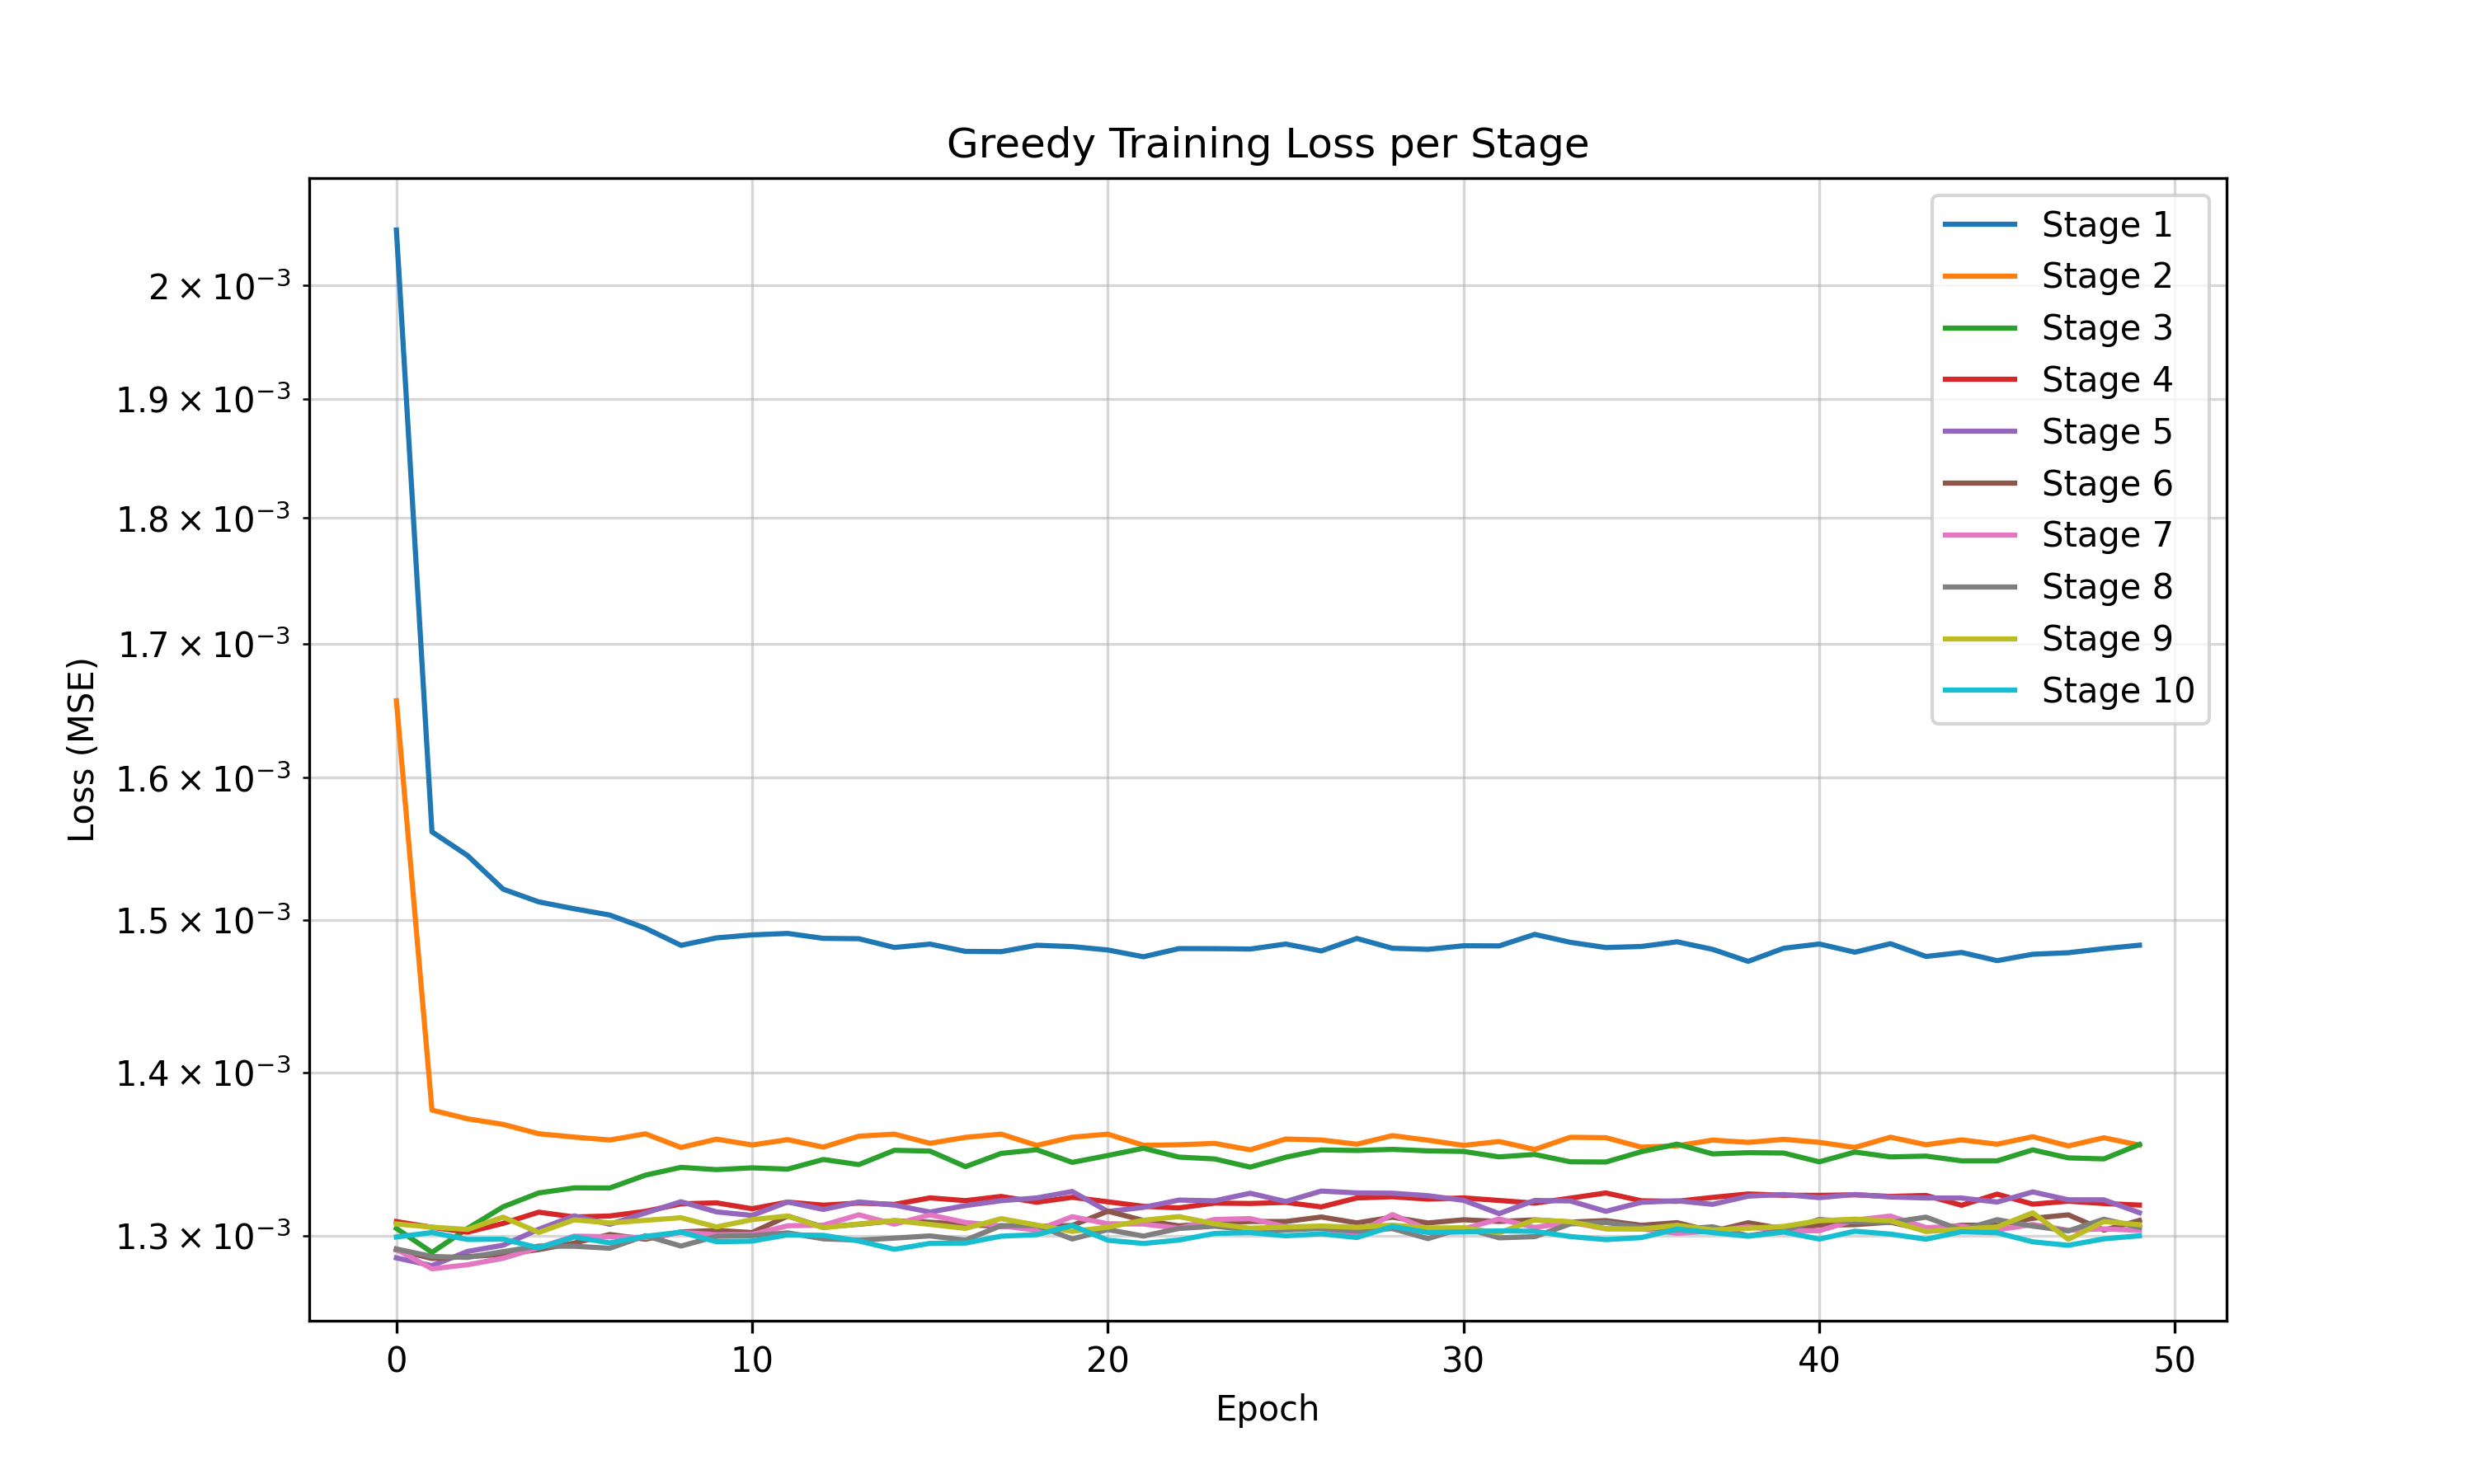
\includegraphics[width=\linewidth]{images/loss_plot.png}
        \caption{Soft-Threshold Loss}
    \end{subfigure}
    \hfill
    \begin{subfigure}{0.48\linewidth}
        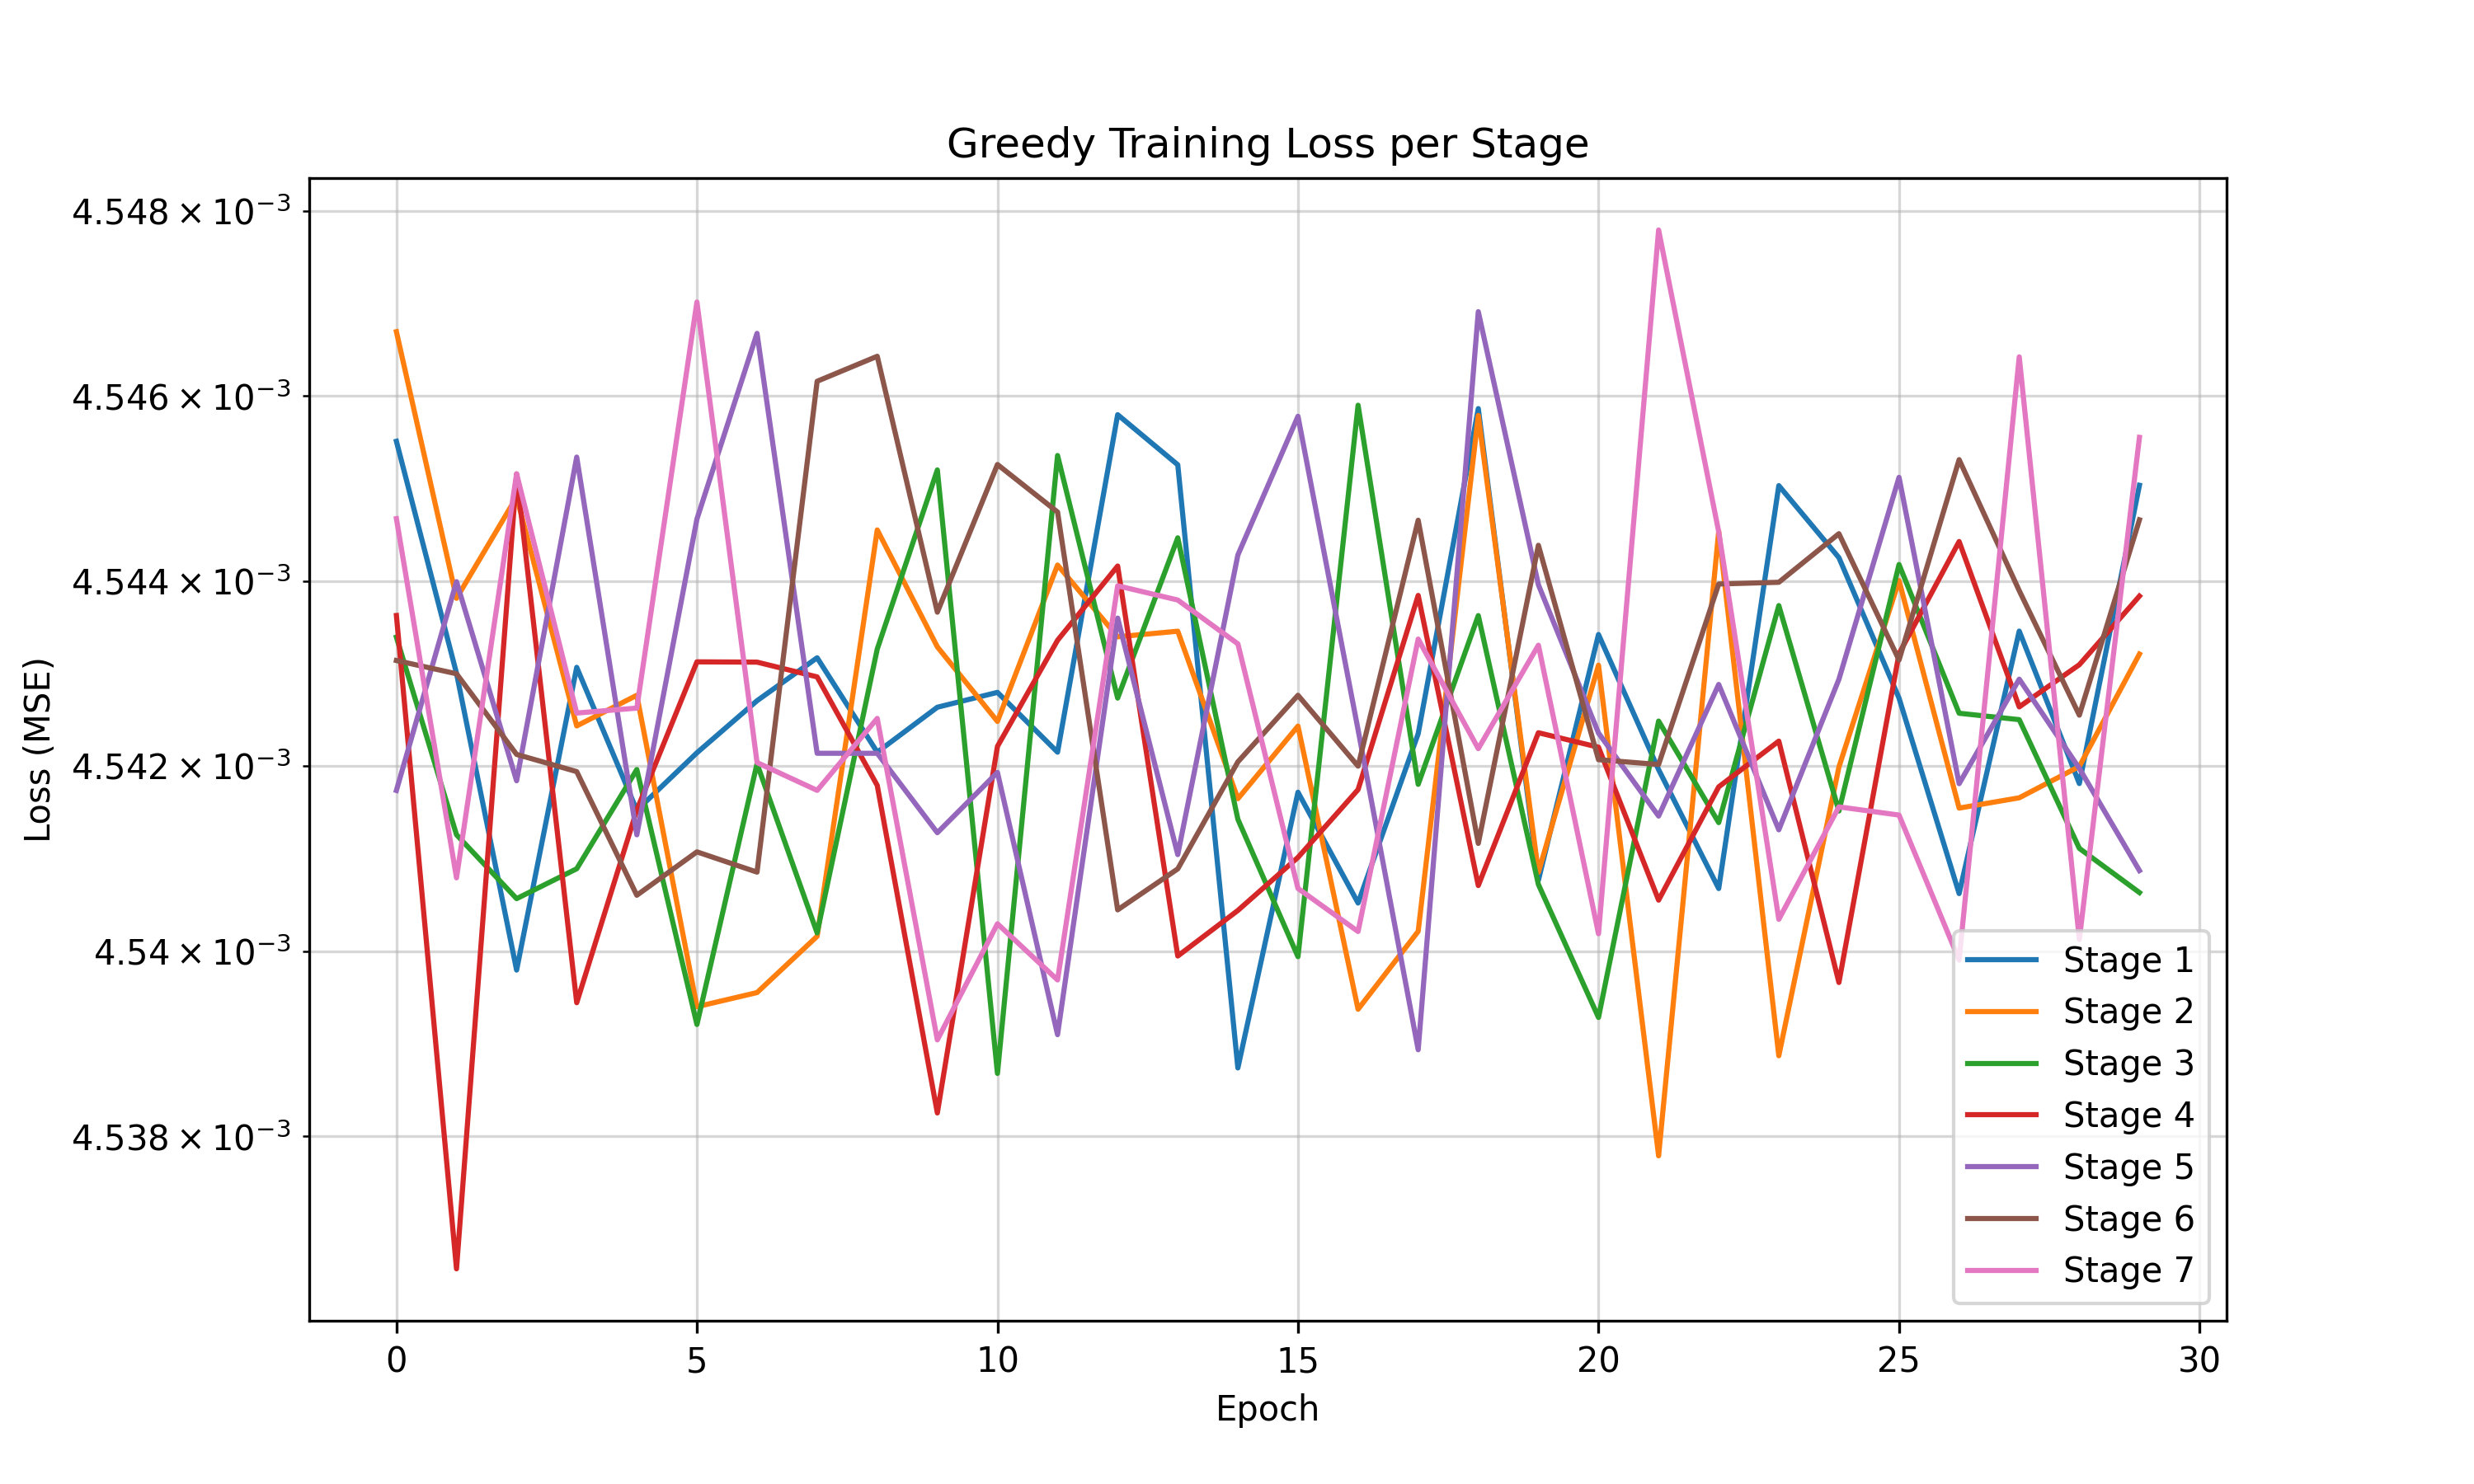
\includegraphics[width=\linewidth]{../ablation_results/fixed_physics/graphs/loss_stages.png}
        \caption{Fixed Physics Loss}
    \end{subfigure}
    \caption{Loss convergence comparison. The "Fixed Physics" model (b) fails to minimize the loss effectively, plateauing at a significantly higher MSE compared to the learnable model (a).}
    \label{fig:loss_comp}
\end{figure}

\end{document}
